\documentclass[12pt,a4paper]{article}
\usepackage[a4paper,top=1.5cm, bottom=1.5cm, left=1.5cm, right=1.5cm]{geometry}
\usepackage[T2A]{fontenc}
\usepackage[utf8]{inputenc}
\usepackage[russian]{babel}
\usepackage{amsmath}
\usepackage{amssymb}
\usepackage{hyperref}
\usepackage{graphicx}
\usepackage{floatrow}
\usepackage{booktabs}
\usepackage{wrapfig}
\usepackage{indentfirst}
\usepackage{lipsum}
\usepackage{subcaption}
\usepackage{float}
\usepackage{derivative}
\usepackage{enumitem}
\restylefloat{table}

\newcommand{\figref}[1]{(см. рис. \ref{#1})}
\newcommand{\e}[1]{\text{$\cdot10^{#1}$}}

\title{Лабораторная работа 3.1.3\\ Измерение магнитного поля Земли}
\author{Симанкович Александр \\ Б01-104}
\date{15.09.2022}

\begin{document}
	\maketitle
	
	\section*{Аннотация}
	
	В работе изучены свойства постоянных неодимовых магнитов (NdFeB) и исследована индукция магнитного поля Земли. Измерены остаточная индукция магнитов $B_r = (7.84 \pm 0.17) \; \text{кГс}$, вертикальная  $B_\parallel = (0.169 \pm 0.012) \cdot 10^5 \; \text{нТл}$ и горизонтальная $ B_{\perp} = (1.14 \pm 0.14) \cdot 10^5 \; \text{нТл}$ составляющие магнитного поля Земли вблизи г. Долгопрудный ($56^\circ$N, $37 ^\circ$E).
	
	\vspace{10pt}
	\noindent\textbf{Ключевые слова}: постоянные магниты, геомагнетизм.
	
	\section*{Введение}
	
	Магнитное поле Земли является слоем защиты от солнечного излучения. Также оно играет ключевую роль в вопросах навигации. Изучение магнитного поля Земли начались еще в XV веке, но до сих пор нет точной теории, его описывающей. На данный момент основной теорией является теория динамо.\footnote{
		\href{https://web.archive.org/web/20070221094040/http://setiathome.berkeley.edu/~pauld/etc/210BPaper.pdf}{Dynamo Theory and Earth's magnetic Field}
	}
	Для численных расчетов используется модель \textbf{IGRF-13}.\footnote{
		\href{https://earth-planets-space.springeropen.com/articles/10.1186/s40623-020-01288-x}
		{International Geomagnetic Reference Field: the thirteenth generation}
	}

	Данная работа была проведена в рамках учебного исследовательского курса в Московском физико-техническом институте. В работе изучаются свойства постоянных неодимовых магнитов и предпринимается попытка исследовать магнитное поле Земли с их помощью.
	
	\section*{Теоретическая модель}
	
	Для начала приведем общие сведения и базовые расчетные формулы.
	
	Магнитный момент $\mathfrak{m}$ тонкого витка площадью $S$ с током $I$:
	$$ \mathfrak{m} = IS \quad \text{(СИ)}, \qquad \mathfrak{m} = \frac{1}{c} IS \quad \text{(СГС)} .$$
	Магнитное поле точечного диполя:
	\begin{equation}
		\label{eq:magnet_dipole}
		\textbf{B}_{\text{дип}} = \frac{\mu_0}{4 \pi} \left( \frac{3(\mathfrak{m} \cdot \textbf{r})\textbf{r}}{r^5} - \frac{\mathfrak{m}}{r^3} \right) \quad (\text{СИ}), \qquad
		\textbf{B}_{\text{дип}} = \frac{3(\mathfrak{m} \cdot \textbf{r})\textbf{r}}{r^5} - \frac{\mathfrak{m}}{r^3} \quad (\text{СГС}) .
	\end{equation}
	Во внешнем магнитном поле с индукцией $\textbf{B}$ на точечный магнитный диполь $\mathfrak{m}$ действует механический момент сил:
	\boldmath
	$$ \mathcal{M} = [\mathfrak{m} \times B] .$$
	\unboldmath
	Потенциальная энергия диполя во внешнем магнитном поле:
	$$ W = -(\mathfrak{m} \cdot \boldsymbol{B}) .$$
	Сила, действующая на диполь в неоднородном поле:
	$$ \boldsymbol{F} = - \nabla W = (\mathfrak{m} \cdot \nabla) \boldsymbol{B}. $$
	В частности, проекция на ось  $x$:
	$$ F_{x} = \mathfrak{m}_x \pdv{B_x}{x}
	+ \mathfrak{m}_y \pdv{B_x}{y}
	+ \mathfrak{m}_z \pdv{B_x}{z}$$
	Cила взаимодействия двух точечных диполей в случае $\mathfrak{m}_{1,2} \parallel \boldsymbol{r} $:
	$$ F_{12} = \mathfrak{m}_1 \pdv{B_2}{r} = -6 \frac{\mathfrak{m_1} \mathfrak{m_2}}{r^4} \quad \text{(CГС)}. \qquad
	F_{12} = - 6 \frac{\mu_0}{4 \pi} \frac{\mathfrak{m_1} \mathfrak{m_2}}{r^4} \quad \text{(СИ)}$$
	Cила взаимодействия двух точечных диполей в случае $\mathfrak{m}_{1,2} \perp \boldsymbol{r} $:
	$$ F_{12} = 3 \frac{\mathfrak{m_1} \mathfrak{m_2}}{r^4} \quad \text{(CГС)}. \qquad
	F_{12} = 3 \frac{\mu_0}{4 \pi} \frac{\mathfrak{m_1} \mathfrak{m_2}}{r^4} \quad \text{(СИ)}$$
	
	\subsection*{Магниты}
	
	В работе используются неодимовые магниты в форме шариков.
	Для равномерно намагниченного магнитожесткого шарика магнитное поле может быть вычислено точно. На расстояниях $r > R$ оно совпадает с полем точечного магнитного диполя \eqref{eq:magnet_dipole}. В случае $r < R$ из непрерывности нормальной компоненты индукции на поверхности шара $B_0$:
	$$ \boldsymbol{B}_0 = \frac{2\mathfrak{m}}{R^3} \quad (\text{СГС}) \qquad 
	\boldsymbol{B}_0 = \frac{\mu_0 \mathfrak{m}}{2 \pi R^3} \quad (\text{СИ}). $$
	Введем \textit{намагниченность} $\boldsymbol{M} $:
	$$ \mathfrak{m} = \boldsymbol{M} V,$$
	где $V$ -- объем магнита.
	Также введем \textit{остаточную индукцию} $\boldsymbol{B}_r$:
	$$ \boldsymbol{B}_r = 4 \pi \boldsymbol{M} \quad (\text{СГС}) \qquad
	\boldsymbol{B}_r = \mu_0 \boldsymbol{M} \quad (\text{СИ}). $$
	$\boldsymbol{B}_p$ -- индукция на полюсах. Так как индукция на полюсах направлена по нормали, то $B_p = B_0$. Тогда для нее выполняется:
	$$ \boldsymbol{B_p} = \boldsymbol{B_0} = \frac{2}{3} \boldsymbol{B_r}. $$
	
	\section*{Методика эксперимента}
	
	\subsection*{Оборудование и приборы}
	\begin{itemize}[itemsep = 0pt, parsep=0pt]
		\item неодимовые магниты;
		\item тонкая нить для изготов­ления крутильного маятника;
		\item медная проволока;
		\item электронные весы;
		\item секундомер;
		\item измеритель магнитной индукции AKTAKOM ATE-870;
		\item штангенциркуль;
		\item брусок, линейка и штатив из немагнитных материалов;
		\item набор гирь и разновесов;
	\end{itemize}
	
	\subsection*{Магнитный момент шариков}
		
	\subsubsection*{Метод А}
	
	\begin{wrapfigure}{r}{0.35\textwidth}
		\vspace{-0pt}
		\center{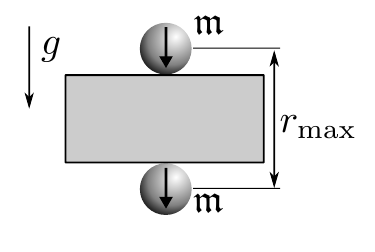
\includegraphics[width=\linewidth]{res/method_A.png}}
		\caption{Определения магнитного момента шарика (Метод A).}
		\label{img:method_a}
	\end{wrapfigure}
	Величину магнитного момента $\mathfrak{m}$ двух
	одинаковых шариков можно рассчитать, зная их массу $m$ и определив максимальное расстояние $r_{max}$, на котором они ещё удерживают друг друга в поле силы тяжести.
	$$ \mathfrak{m} = \sqrt{\frac{mgr_{max}^4}{6}} \quad (\text{СГС}) $$
	
	При данном способе измерений возникает несколько проблем. Во-первых, шарики сложно ориентировать полюсами строго вертикально, что сильно снижает силу взаимодействия. Во-вторых, сжатие бумаги. Неизвестно, насколько сжимается бумага под силой взаимодействия шариков, поэтому точное расстояние также трудноопределимо. Данные недостатки могут значительно исказить результаты измерений.
	
	\subsubsection*{Метод Б}

	\begin{wrapfigure}{r}{0.35\textwidth}
		\vspace{-20pt}
		\center{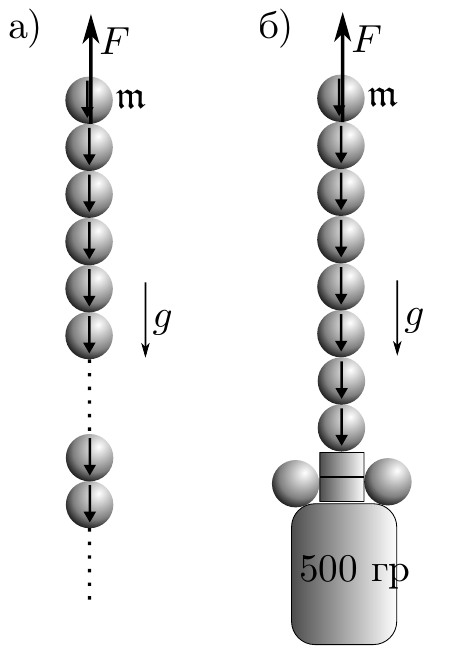
\includegraphics[width=0.5\linewidth]{res/method_B.png}}
		\caption{Определения магнитного момента шарика (Метод Б).}
		\label{img:method_b}
		\vspace{-10pt}
	\end{wrapfigure}
	Величину магнитного момен­та шариков можно определить также по си­ле их сцепления. Она определяется как сила для разрыва двух магнитных шариков. Для этого можно построить цепочку из шариков и определить, при какой длине она разорвется \figref{img:method_a}. Также нижнюю часть цепочки шаров можно заменить на массивный груз.
	
	Сила сцепления одинаковых шариков:
	$$ F_0 = \frac{3\mathfrak{m}^2}{8 R^4}. $$
	Посчитав силы взаимодействия 1-го и остальных шариков и отбросив шарики ниже 4-го получим:
	$$ F \approx 1.08 F_0. $$
	
	Данный метод не имеет недостатков, характерных для метода А. При измерении фиксировать цепочку нужно за верхний шарик. При этом даже если при фиксации удерживать второй шарик, погрешность увеличится не более, чем на 4\%.
		
	\subsection*{Измерение индукции магнитного поля Земли}
	
	\subsubsection*{Горизонтальная составляющая}
	\begin{wrapfigure}{R}{0.4\textwidth}
		\vspace{30pt}
		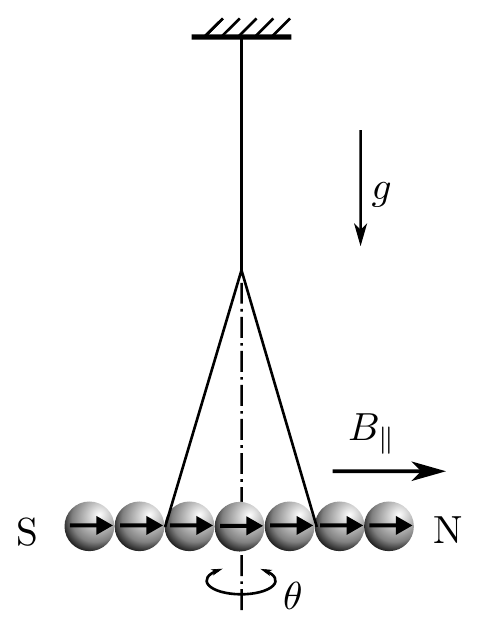
\includegraphics[width=0.8\linewidth]{res/horizontal.png}
	\end{wrapfigure}
 
	Магнитная 'стрелка' образована из $n$ сцепленных друг с другом противоположными полюсами шариков и с помощью $\Lambda$-образного подвеса подвешена в горизонтальном положении. При отклонении 'стрелки' на угол $\theta$ от равновесного положения в горизонтальной плоскости возникают крутильные колебания вокруг вертикальной оси, проходящей через середину стрелки. При малых амплитудах уравнение колебаний
	стрелки имеет вид:
	$$ J_n \dfrac{d^2 \theta}{dt^2} + \mathfrak{m}_0 B_{\parallel} \theta = 0, $$ 
	где $\mathfrak{m}_0 = n \mathfrak{m}$ -- магнитный момент стрелки, $B_{\parallel}$ -- горизонтальная составляющая магнитного поля Земли, $J_n \approx \dfrac{1}{3}n^3 m R^3$, тогда период колебаний $T = kn$, где $k = \pi \sqrt{\dfrac{md^2}{3 \mathfrak{m} B_h}}$. Измеряя зависимость $T=T(n)$, находится $B_{\parallel}$:
	$$ B_{\parallel} = \dfrac{\pi^2 m d^2}{3k^2\mathfrak{m}}. $$
	
	\subsubsection*{Вертикальная составляющая}
	
	\begin{wrapfigure}{R}{0.6\textwidth}
		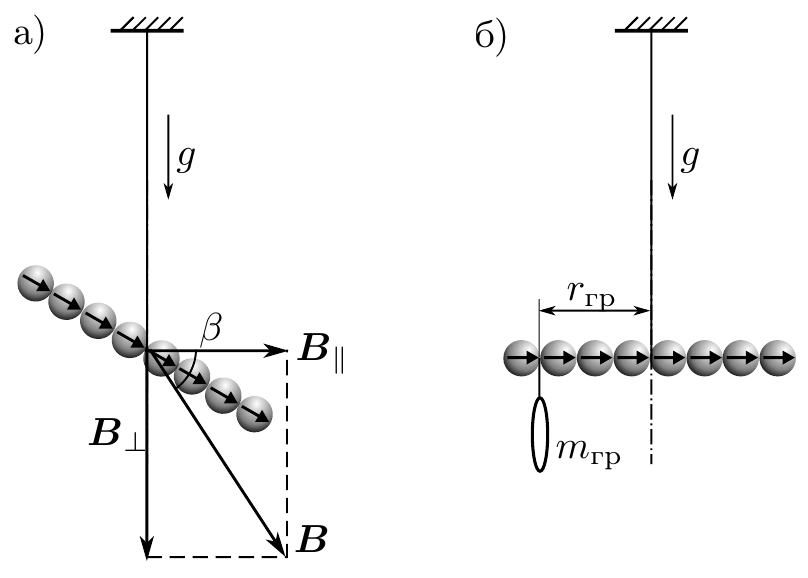
\includegraphics[width=0.8\linewidth]{res/vertical.png}
		\vspace{30pt}
	\end{wrapfigure}
	
	Магнитная «стрелка», составленная из чётного числа
	шариков и подвешенная на тонкой нити за середину, расположится не горизонтально, а под некоторым, отличным от нуля, углом к горизонту. Это связано с тем, что вектор $\boldsymbol{B}$ индукции магнитного поля Земли в общем случае не горизонтален, а образует с горизонтом
	угол $\beta$, зависящим от географической широты $\varphi$
	места, где проводится опыт. Величина угла $\beta$
	называется магнитным наклонением.
	
	С помощью небольшого дополнительного грузика «стрелку» можно «выровнять». Момент $\mathcal{M}$ силы тяжести уравновешивающего груза пропорционален числу $n$ шариков, образующих магнитную 'стрелку':
	$$\mathcal{M}(n) = m_{\text{гр}} g r_{\text{гр}} = n \mathfrak{m} B_\perp. $$
	
	\subsection*{Недостатки методики измерений}
	
	Цепочка из шариков при подвешивании деформируется. Это было частично решено созданием 'корпуса' для шариков из бумаги.
	
	При измерении вертикальной составляющей возникли еще несколько проблем. Дополнительный грузик должен быть очень легким, поэтому в качестве грузика использовали бумагу. Точность выкладывания бумаги на 'стрелку' очень невелика. Также само положение крепления стрелки могло смещаться (поскольку шарики находились в 'корпусе'), что приводило к разбалансированию стрелки.
	
	\section*{Результаты}
	
	Измерим диаметр шариков микрометром:
	$$ d = (6.29 \pm 0.01) \; \text{мм} \quad \Rightarrow \quad r = (3.145 \pm 0.01) \; \text{мм}. $$
	
	Измерим массу шариков на весах. Положим на весы через пластиковую подставку 20 шариков. Результаты:
	$$ m_\Sigma = (16.633 \pm 0.001) \; \text{г} \quad \Rightarrow \quad m = (0.832 \pm 0.001) \; \text{г}. $$
	
	Измерим индукцию поля шариков на полюсах $B_p$ с помощью тесламетра:
	$$ B_p = (270 \pm 16) \; \text{мТл} = (2.70 \pm 0.16) \; \text{кГс}. $$
	Ошибка такого измерения в действительности сильно зависит от точности направления полюса шарика. Также сильно влияет малый размер шарика, поскольку детектор тесламетра имеет размеры $l \approx 3 \; \text{мм}$ и даже малый сдвиг детектора может сильно исказить значение.
	
	Укажем также табличные значения остаточной индукции $B_r$ для неодимовых магнитов:
	$$ B_r^{ref} = (10 \div 13) \; \text{кГс}. $$
	
	\subsubsection*{Метод А}
	
	Подложим между шариками брусок из немагнитного материала. Далее будем подкладывать листы бумаги, пока шарики не перестанут удерживать друг друга неподвижно.
	$$ r_{max} = (18.59 \pm 0.05 ) \; \text{мм}. $$
	
	Рассчитаем магнитный момент одного магнита $\mathfrak{m}$:
	$$ \mathfrak{m} = \sqrt{\frac{mgr_{max}^4}{6}} = \sqrt{\frac{0.8317 \cdot 9.81 \cdot 10^2 \cdot 1.859^4}{6}} = (40.3 \pm 0.2) \; \text{Гс} \cdot \text{см}^3. $$
	
	Рассчитаем параметры магнита:
	$$ B_p = \frac{2\mathfrak{m}}{R^3} = (2.59 \pm 0.03) \; \text{кГс}. $$
	
	$$ M = \frac{\mathfrak{m}}{V} = (309 \pm 3) \; \text{Гс}. $$
	
	$$ B_r = \frac{3}{2} B_p = (3.89 \pm 0.04) \; \text{кГс}. $$
	
	Результаты сходятся с измерением тесламетром. При этом значения $B_r$ не сходится с табличным. Могут иметь место два исхода: 1) шарики потеряли намагниченность; 2) измерения как методом А, так и тесламетром, неточны.
	
	\subsubsection*{Метод Б}
	
	Рассчитаем $\mathfrak{m}$:
	$$ \mathfrak{m} = \sqrt{\frac{8 F {R}^4}{3 \cdot 1.08}} = (81.3 \pm 1.5) \; \text{Гс} \cdot \text{см}^3. $$
	
	Рассчитаем параметры магнита:
	$$ B_p = \frac{2\mathfrak{m}}{R^3} = (5.23 \pm 0.11) \; \text{кГс}. $$
	
	$$ M = \frac{\mathfrak{m}}{V} = (624 \pm 13) \; \text{Гс}. $$
	
	$$ B_r = \frac{3}{2} B_p = (7.84 \pm 0.17) \; \text{кГс}. $$
	
	Результаты не сходятся с измерением тесламетром и с методом А. Метод Б имеет вышеописанные преимущества перед методом А, измерение тесламетром также может иметь невысокую точность. При этом результат показывает значение остаточной индукции $B_r$ меньшее, чем справочное, но близкое к нему. По этой причине для последующих расчетов выбраны результаты метода Б.
	
	\subsubsection*{Горизонтальная составляющая магнитного поля Земли}
	
	Свернем магнитную стрелку из шариков в кольцо и измерим период колебаний: $ T = 92 \; \text{с}$. Пусть $\xi$ -- упругость нити на кручение. Тогда:
	$$ T = 2 \pi \sqrt{\frac{J}{\xi}} \quad \Rightarrow \quad \xi = 4 \pi^2 \frac{J}{T^2}.$$
	Если период колебаний кольца на нити много больше периода колебаний стрелки, то влиянием нити можно пренебречь.
	
	%\begin{table}[H]
	%	\caption{Результаты измерений для горизонтальной составляющей магнитного поля Земли}
	%	\input{gen/horizontal.tex}
	%\end{table}

	При измерениях колебаний 'стрелки' время колебаний на порядок меньше, значит влияние упругости нити меньше на два порядка.
	
	\begin{figure}[H]
		\includegraphics[]{gen/horizontal_Tn.pdf}
		\caption{Зависимость механического момента от числа шариков}
	\end{figure}
	
	\begin{table}[H]
		\caption{Параметры графика $T(n)$}
		\input{gen/horizontal_mnk.tex}
	\end{table}
	
	Рассчитаем значение горизонтальной составляющей магнитного поля Земли:
	$$ B_{\parallel} = \dfrac{\pi^2 m d^2}{3k^2\mathfrak{m}} = (0.169 \pm 0.012) \; \text{Гс}. $$
	
	\subsubsection*{Вертикальная составляющая магнитного поля Земли}
	
	Проведем измерения в соответствии с методикой, описанной выше.
	
	%\begin{table}[H]
	%	\caption{Результаты измерений для вертикальной составляющей магнитного поля Земли}
	%	\input{gen/vertical.tex}
	%\end{table}
	
	\begin{figure}[H]
		\includegraphics[]{gen/vertical_Mn.pdf}
		\caption{Зависимость механического момента от числа шариков}
	\end{figure}
	
	\begin{table}[H]
		\caption{Параметры графика $M(n)$}
		\input{gen/vertical_mnk.tex}
	\end{table}
	
	Рассчитаем значение вертикальной составляющей магнитного поля Земли:
	$$ B_{\perp} = \frac{k}{\mathfrak{m}} = (1.14 \pm 0.14) \; \text{Гс}. $$
	
	Рассчитаем также наклонение $\beta$ и полную величину $B$ магнитного поля Земли:
	
	$$ \beta = \arctan{\frac{B_\perp}{B_\parallel}} = 81 ^\circ \; \text{вниз} \qquad B = (1.16 \pm 0.17) \; \text{Гс}.$$
	\section*{Заключение и выводы}
	
	Данная работа подтверждает существование магнитного поля Земли и наличие существенного магнитного наклонения на широте $56 ^\circ$ и долготе $37 ^\circ$ (г. Долгопрудный).
	
	Получено значение остаточной индукции неодимовых магнитов $B_r = (7.84 \pm 0.17) \; \text{кГс}$. Данный результат по порядку совпадает со справочным $B_r^{ref} = (10 \div 13) \; \text{кГс}$ и может объяснятся потерей намагниченности со временем.
	
	Оценены значения горизонтальной $B_\parallel = (0.169 \pm 0.012) \; \text{Гс} = (0.169 \pm 0.012) \cdot 10^5 \; \text{нТл}$ и вертикальной $ B_{\perp} = (1.14 \pm 0.14) \; \text{Гс} = (1.14 \pm 0.14) \cdot 10^5 \; \text{нТл}$ составляющих магнитного поля Земли. Значение магнитного наклонения $\beta = 81 ^\circ$, модуль магнитного поля земли $B = (1.16 \pm 0.17) \; \text{Гс}$.
	
	Модель магнитного поля Земли \textbf{IGRF-13}
	для точки в районе г. Долгопрудного дает $B_\parallel = 0.16550 \cdot 10^5 \; \text{нТл}$, $B_\perp = 0.50277 \cdot 10^5 \; \text{нТл}$, магнитноe наклонениe $\beta = 71.780 ^\circ$ вниз, модуль магнитного поля $B = 0.52907 \cdot 10^5 \; \text{нТл}$. Сравнение с данной моделью дает сильное расхождение в вертикальной компоненте. Это объясняется недостатками методики измерений.
	
	Для улучшения результатов есть несколько возможностей. Можно улучшить методику измерения поля магнитов: использовать немагнитный фиксатор для закрепления магнита в методе Б и при измерении тесламетром. При измерении горизонтальной и вертикальной составляющей магнитного поля Земли лучше использовать плоские магниты, которые не будут создавать прогиба 'стрелки'. Также для закрепления стрелки можно использовать карданов подвес, избавляющий от нежелательных моментов силы. Подвешивание противовеса при измерении вертикальной составляющей упростится, если зажимать противовес между магнитами.
	
\end{document}